\documentclass{standalone}
\usepackage{tikz}

% (c) Dave Snowden


\begin{document}
    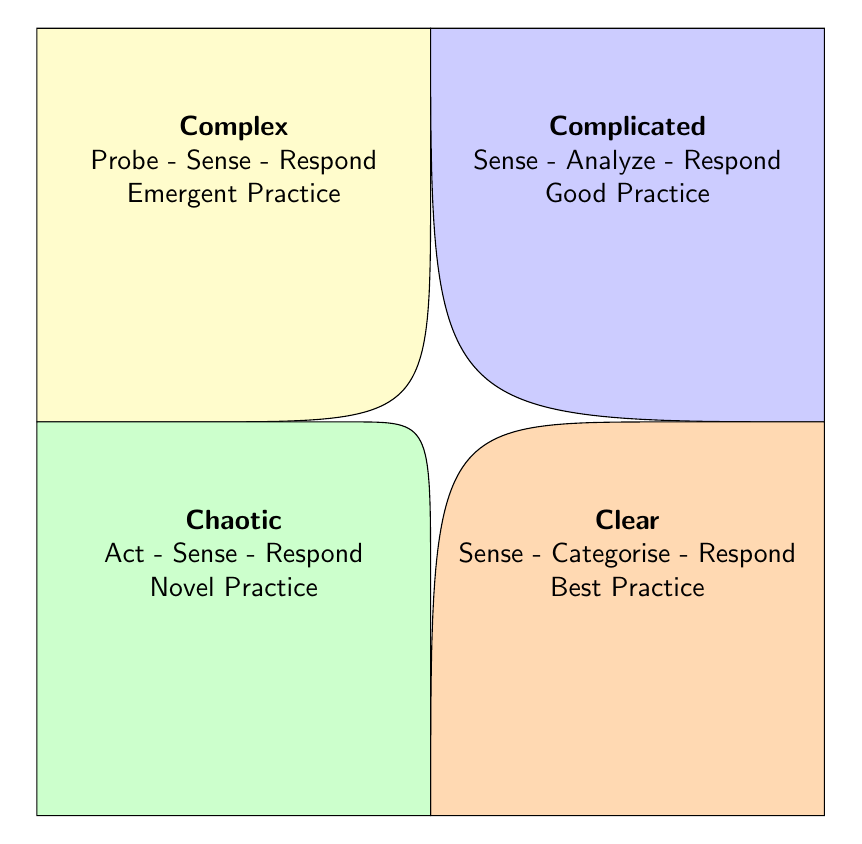
\begin{tikzpicture}
        \tikzset{every node/.style={text width=5cm,anchor=north,align=center,font=\sffamily}};
        % \draw (0,0) rectangle (10,10);
        \path[draw,fill=yellow!20] (0,5) -- (2,5) .. controls (5,5) .. (5,8) -- (5,10) -- (0,10) -- (0,5) -- cycle ;
        \path[draw,fill=blue!20] (5,10) -- (10,10) -- (10,5) .. controls (5,5)  .. (5,10) -- cycle;
        \path[draw,fill=orange!30] (10,0) -- (10,5) -- (8,5) .. controls (5,5)  ..  (5,0) -- cycle;
        \path[draw,fill=green!20] (0,0) -- (0,5) -- (4,5) .. controls (5,5)  .. (5,3) -- (5,0) -- cycle;
        \node at (2.5,4) {\textbf{Chaotic}\\ Act - Sense - Respond\\ Novel Practice};
        \node at (2.5,9) {\textbf{Complex}\\ Probe - Sense - Respond\\ Emergent Practice};
        \node at (7.5,4) {\textbf{Clear}\\ Sense - Categorise - Respond\\ Best Practice};
        \node at (7.5,9) {\textbf{Complicated}\\ Sense - Analyze - Respond\\ Good Practice };
    \end{tikzpicture}
\end{document}